% ----- Consignes exo 1 ----- %
\begin{td-exo}[Bouillabaisse]\,\\ % 1
    Je possède huit espèces de poissons. Dans le tableau c-dessous, une croix indique que deux poissons des espèces correspondantes ne peuvent cohabiter.
    \begin{center}
        \begin{tabular}{|c|c|c|c|c|c|c|c|c|} % chktex 44
            \hline  % chktex 44
            \ & Anchois & Baudroie & Calmar & Dorade & Espadon & Flétan & Goujon & Hareng \\
            \hline % chktex 44
            Anchois & \ & \(\times\) & \(\times\) & \(\times\) & \ & \ & \(\times\) & \(\times\) \\
            \hline % chktex 44
            Baudroie & \(\times\) & \ & \ & \ & \(\times\) & \(\times\) & \(\times\) & \ \\
            \hline % chktex 44
            Calmar & \(\times\) & \ & \ & \(\times\) & \ & \(\times\) & \(\times\) & \ \\
            \hline % chktex 44
            Dorade & \(\times\) & \ & \(\times\) & \ & \(\times\) & \ & \ & \(\times\) \\
            \hline % chktex 44
            Espadon & \ & \(\times\) & \ & \(\times\) & \ & \(\times\) & \(\times\) & \ \\
            \hline % chktex 44
            Flétan & \ & \(\times\) & \(\times\) & \ & \(\times\) & \ & \ & \ \\
            \hline % chktex 44
            Goujon & \(\times\) & \(\times\) & \(\times\) & \ & \(\times\) & \ & \ & \ \\
            \hline % chktex 44
            Hareng & \(\times\) & \ & \(\times\) & \(\times\) & \ & \ & \ & \ \\
            \hline % chktex 44
        \end{tabular}
    \end{center}
    Combien faut-il au minimum que j'achète d'aquariums?
\end{td-exo}

% ----- Solutions exo 1 ----- %
\iftoggle{showsolutions}{
	\begin{td-sol}[]\,\\ % 1
		On peut représenter le problème avec le graphe \(G\) suivant:

        \vspace{0.2cm}
        \ffigbox[\FBwidth]{%
\caption{\centering Graphe de poissons}\label{Fig:td_5_ex_1_1}
}{
    \fbox{
        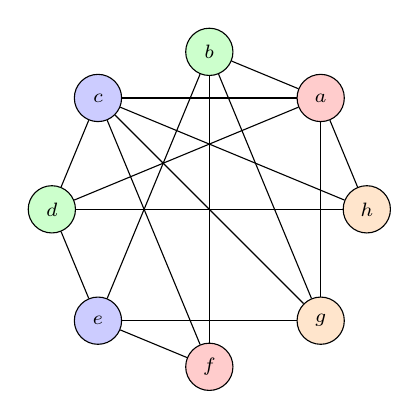
\begin{tikzpicture}[scale=1, 
            main node/.style={circle, draw, fill=blue!20, inner sep=1pt, font=\scriptsize, minimum size=6mm}, 
            cola node/.style={circle, draw, fill=red!20, inner sep=1pt, font=\scriptsize, minimum size=6mm}, 
            colb node/.style={circle, draw, fill=green!20, inner sep=1pt, font=\scriptsize, minimum size=6mm}, 
            colc node/.style={circle, draw, fill=blue!20, inner sep=1pt, font=\scriptsize, minimum size=6mm}, 
            cold node/.style={circle, draw, fill=orange!20, inner sep=1pt, font=\scriptsize, minimum size=6mm}]
            % le cercle de départ 
            % \draw (0, 0) circle [radius=2];
            
            % les sommets initiaux
            \node[cola node] (a) at (45:2)  {\(a\)};
            \node[colb node] (b) at (90:2)  {\(b\)};
            \node[colc node] (c) at (135:2) {\(c\)};
            \node[colb node] (d) at (180:2){\(d\)};
            \node[colc node] (e) at (225:2){\(e\)};
            \node[cola node] (f) at (270:2){\(f\)};
            \node[cold node] (g) at (315:2){\(g\)};
            \node[cold node] (h) at (0:2){\(h\)};
            % ahcd
            \draw (a) -- (b);
            \draw (a) -- (c);
            \draw (a) -- (d);
            \draw (a) -- (g);
            \draw (a) -- (h);

            \draw (b) -- (e);
            \draw (b) -- (f);
            \draw (b) -- (g);

            \draw (c) -- (d);
            \draw (c) -- (f);
            \draw (c) -- (g);
            \draw (c) -- (h);

            \draw (d) -- (e);
            \draw (d) -- (h);

            \draw (e) -- (f);
            \draw (e) -- (g);
        \end{tikzpicture}
    }
}

        où le sommet \(i\) correspond au poisson qui commence par la lettre \(i\). On voit que les sommets \(acdh\) forment un \(K_4\) donc \(\chi(G) \geq 4\). De plus, on a trouvé une 4-coloration donc \(\chi(G)=4\).

	\end{td-sol}
}{}


% ----- Consignes exo 2 ----- %
\begin{td-exo}[Crayonnage]\,\\ % 2
    Déterminer le nombre chromatique des deux graphes suivants:
    
    \vspace{0.2cm}
    \begin{figure}[H]
        \CenterFloatBoxes{}
        \begin{floatrow}
            % Figure 1
\ffigbox[\FBwidth]{
\caption{\centering Graphe \(G_1\) dé départ}\label{Fig:td5ex2c1}
}{
    \fbox{
        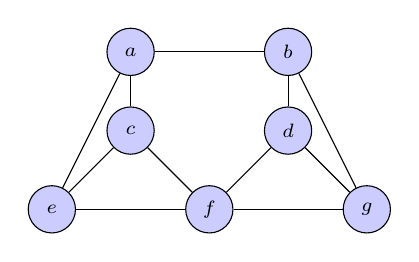
\begin{tikzpicture}[scale=1,
            main node/.style={circle, draw, fill=blue!20, inner sep=1pt, font=\scriptsize, minimum size=6mm}]
            \node[main node] (a) at (0, 0) {\(a\)};
            \node[main node] (b) at (2, 0) {\(b\)};
            \node[main node] (c) at (0, -1) {\(c\)};
            \node[main node] (d) at (2, -1) {\(d\)};
            \node[main node] (e) at (-1, -2) {\(e\)};
            \node[main node] (f) at (1, -2) {\(f\)};
            \node[main node] (g) at (3, -2) {\(g\)};
            
            \draw (a) -- (b);
            \draw (a) -- (c);
            \draw (a) -- (e);

            \draw (b) -- (d);
            \draw (b) -- (g);

            \draw (c) -- (e);
            \draw (c) -- (f);

            \draw (d) -- (f);
            \draw (d) -- (g);

            \draw (e) -- (f);

            \draw (f) -- (g);
        \end{tikzpicture}
    }
}

            % Figure 1
\ffigbox[\FBwidth]{
\caption{\centering Graphe \(G_2\) dé départ}\label{Fig:td5ex2c2}
}{
    \fbox{
        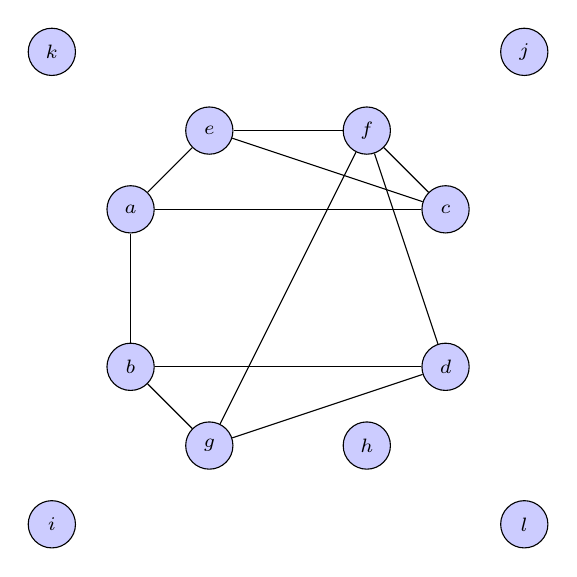
\begin{tikzpicture}[scale=1,
            main node/.style={circle, draw, fill=blue!20, inner sep=1pt, font=\scriptsize, minimum size=6mm}]
            \node[main node] (a) at (-2, 1) {\(a\)};
            \node[main node] (b) at (-2, -1) {\(b\)};
            \node[main node] (c) at (2, 1) {\(c\)};
            \node[main node] (d) at (2, -1) {\(d\)};
            \node[main node] (e) at (-1, 2) {\(e\)};
            \node[main node] (f) at (1, 2) {\(f\)};
            \node[main node] (g) at (-1, -2) {\(g\)};
            \node[main node] (h) at (1, -2) {\(h\)};
            \node[main node] (i) at (-3, -3) {\(i\)};
            \node[main node] (j) at (3, 3) {\(j\)};
            \node[main node] (k) at (-3, 3) {\(k\)};
            \node[main node] (l) at (3, -3) {\(l\)};


            
            
            \draw (a) -- (b);
            \draw (a) -- (c);
            \draw (a) -- (e);

            \draw (b) -- (d);
            \draw (b) -- (g);

            \draw (c) -- (e);
            \draw (c) -- (f);

            \draw (d) -- (f);
            \draw (d) -- (g);

            \draw (e) -- (f);

            \draw (f) -- (g);
        \end{tikzpicture}
    }
}
        \end{floatrow}
    \end{figure}
    % insert graphs here
\end{td-exo}

% ----- Solutions exo 2 ----- %
\iftoggle{showsolutions}{
	\begin{td-sol}[]\,\\ % 2
		Le graphe \(G_1\) a pour nombre chromatique 4. Comme tout a l'heure, comme il existe un cycle impair dans \(G_1\), on a \(\chi(G_1) \geq 3\). On ne peut pas trouver de 3-coloration mais on a une 4-coloration donc \(\chi(G_1)=4\):

        \vspace{0.2cm}
        % Figure 1
\ffigbox[\FBwidth]{
\caption{\centering Graphe \(G_1\) colorié}\label{Fig:td5ex2c3}
}{
    \fbox{
        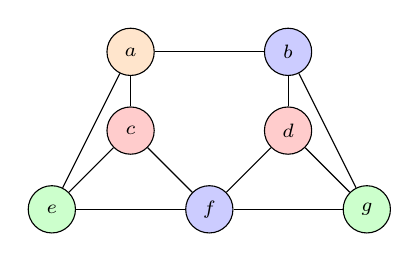
\begin{tikzpicture}[scale=1,
            main node/.style={circle, draw, fill=blue!20, inner sep=1pt, font=\scriptsize, minimum size=6mm}, 
            cola node/.style={circle, draw, fill=red!20, inner sep=1pt, font=\scriptsize, minimum size=6mm}, 
            colb node/.style={circle, draw, fill=green!20, inner sep=1pt, font=\scriptsize, minimum size=6mm}, 
            colc node/.style={circle, draw, fill=blue!20, inner sep=1pt, font=\scriptsize, minimum size=6mm}, 
            cold node/.style={circle, draw, fill=orange!20, inner sep=1pt, font=\scriptsize, minimum size=6mm}]
            \node[cold node] (a) at (0, 0) {\(a\)};
            \node[colc node] (b) at (2, 0) {\(b\)};
            \node[cola node] (c) at (0, -1) {\(c\)};
            \node[cola node] (d) at (2, -1) {\(d\)};
            \node[colb node] (e) at (-1, -2) {\(e\)};
            \node[colc node] (f) at (1, -2) {\(f\)};
            \node[colb node] (g) at (3, -2) {\(g\)};
            
            \draw (a) -- (b);
            \draw (a) -- (c);
            \draw (a) -- (e);

            \draw (b) -- (d);
            \draw (b) -- (g);

            \draw (c) -- (e);
            \draw (c) -- (f);

            \draw (d) -- (f);
            \draw (d) -- (g);

            \draw (e) -- (f);

            \draw (f) -- (g);
        \end{tikzpicture}
    }
}
        
        Le graphe \(G_2\) a pour nombre chromatique 4.
	\end{td-sol}
}{}


% ----- Consignes exo 3 ----- %
\begin{td-exo}[]\,\\ % 3
    Exercise 3 content
\end{td-exo}

% ----- Solutions exo 3 ----- %
\iftoggle{showsolutions}{
	\begin{td-sol}[]\,\\ % 3
		Exercice solution
	\end{td-sol}
}{}


% ----- Consignes exo 1 ----- %
\begin{td-exo}[]\,\\ % 1
    Exercise 1 content
\end{td-exo}

% ----- Solutions exo 1 ----- %
\iftoggle{showsolutions}{
	\begin{td-sol}[]\,\\ % 1
		Exercice solution
	\end{td-sol}
}{}


% ----- Consignes exo 1 ----- %
\begin{td-exo}[]\,\\ % 1
    Exercise 1 content
\end{td-exo}

% ----- Solutions exo 1 ----- %
\iftoggle{showsolutions}{
	\begin{td-sol}[]\,\\ % 1
		Exercice solution
	\end{td-sol}
}{}


% ----- Consignes exo 1 ----- %
\begin{td-exo}[]\,\\ % 1
    Exercise 1 content
\end{td-exo}

% ----- Solutions exo 1 ----- %
\iftoggle{showsolutions}{
	\begin{td-sol}[]\,\\ % 1
		Exercice solution
	\end{td-sol}
}{}


% ----- Consignes exo 1 ----- %
\begin{td-exo}[]\,\\ % 1
    Exercise 1 content
\end{td-exo}

% ----- Solutions exo 1 ----- %
\iftoggle{showsolutions}{
	\begin{td-sol}[]\,\\ % 1
		Exercice solution
	\end{td-sol}
}{}


% ----- Consignes exo 1 ----- %
\begin{td-exo}[]\,\\ % 1
    Exercise 1 content
\end{td-exo}

% ----- Solutions exo 1 ----- %
\iftoggle{showsolutions}{
	\begin{td-sol}[]\,\\ % 1
		Exercice solution
	\end{td-sol}
}{}


